\documentclass[a4paper, 11pt]{article}

\usepackage{davrecipes}

% ----------------------------------------------------------------------------------------------------
%   Title
% ----------------------------------------------------------------------------------------------------
\title{Ricette}
\author{Davide Ponzini}
\date{\today}

% PDF meta-information
\hypersetup{
    pdftitle={Ricette - Davide Ponzini},
    pdfauthor={Davide Ponzini},
    pdfpagemode=FullScreen,
}

% ----------------------------------------------------------------------------------------------------

\begin{document}

% ----------------------------------------------------------------------------------------------------
%   HEADER
% ----------------------------------------------------------------------------------------------------
\makeheader

% ----------------------------------------------------------------------------------------------------
%   TEMPLATE
% ----------------------------------------------------------------------------------------------------
% \begin{recipe}[label=template]{Nome Ricetta}
    \begin{header}
        \portion{5}[piatti]
        \source{Internet}
        \recipedate{Luglio 2023}

        \preparationTime     {\timeM{15}}
        \preparationWait     {\timeM{5}}
        \cookingTime         {\timeM{10}}{Fiamma alta}
        \bakingTimeBottom    {\timeH{1}}{180}
        \bakingTimeTop       {\timeH{1}}{180}
        \bakingTimeTopbottom {\timeH{1}}{180}
        \bakingTimeFan       {\timeH{1}}{180}
    \end{header}

    \begin{introduction}
        Introduzione alla ricetta.
    \end{introduction}

    \begin{ingredients}
    % \begin{ingredients*}        % per ricetta senza step preparazione
        \ingredientSection*{Prima sezione}
        \ingredient[100][g]{Farina}
        \ingredient[2]{Pomodori}
        
        \ingredientSection{Sezione con spazio}
        \ingredient{Sale}
        \ingredient{Pepe}
        
        \ingredientSection*{Sezione senza spazio}
        \ingredient*{Carta forno}
    % \end{ingredients*}
    \end{ingredients}

    \begin{preparation}
        \step Passaggio per preparare la ricetta.
        \step Altro passaggio per preparare la ricetta.
        \step* --- --- --- ---
        \step Ultimo passaggio.
    \end{preparation}

    \begin{suggestion}[2cm]
        \suggestionMark Consiglio da rispettare.
        \suggestionMark Consiglio da rispettare.
    \end{suggestion}

    \begin{hint}
        Note in fondo alla pagina.
    \end{hint}
\end{recipe}


% ----------------------------------------------------------------------------------------------------
%   CONTENT
% ----------------------------------------------------------------------------------------------------
\fakesection{Primi}[Pasta aglio, olio e peperoncino]
\begin{recipe}{Pasta aglio, olio e peperoncino}
    \begin{header}
        \portion{1}
    
        \preparationTime{\timeM{2}}
        \cookingTime{\timeM{11}}{Fiamma alta}
    \end{header}
    
    \begin{ingredients}[5]
        \ingredient[100][g]{Spaghetti}
        \ingredient[1][spicchio]{Aglio}
        \ingredient{Olio}
        \ingredient{Peperoncino}
    \end{ingredients}
    
    \begin{preparation}
        \step Mettere in una padella olio e aglio.
        \step Far rosolare. Infine aggiungere peperoncino.
        \step Cuocere pasta normalmente.
        \step Unire e mescolare.
        \step (Opzionale) Aggiungere del formaggio grattugiato; non mescolare.
    \end{preparation}
\end{recipe}

\begin{recipe}{Pasta pomodoro fresco crudo}
    \begin{header}
        \portion{2}
        \source{Abbate Maria Luisa}
        
        \preparationTime{\timeM{10}}
        \cookingTime{\timeM{11}}{Fiamma alta}
    \end{header}
    
    \begin{ingredients}
        \ingredient[200][g]{Pasta}
        \ingredient[200+][g]{Pomodori (maturi)}
        \ingredient[1][spicchio]{Aglio}
        \ingredient[4-5][foglie]{Basilico}
        \ingredient{Sale}
        \ingredient{Olio}
    \end{ingredients}
    
    \begin{preparation}
        \step Frullare pomodori, aglio, basilico, olio e sale.
        \step Preparare la pasta normalmente.
        \step Unire alla salsa e mescolare.
    \end{preparation}
\end{recipe}

\begin{recipe}{Pasta pomodoro fresco cotto}
    \begin{header}
        \portion{2}
        \source{Abbate Maria Luisa}
        
        \preparationTime{\timeM{10}}
        \cookingTime{\timeM{40+}}{Fiamma medio-alta}[Pomodori]
        \preparationTime{\timeM{10}}
        \cookingTime{\timeM{11}}{Fiamma alta}[Pasta]
    \end{header}
    
    \begin{ingredients}[8]
        \ingredient[200][g]{Pasta}
        \ingredient[250-400+][g]{Pomodori (maturi)}
        \ingredient[2]{Dadi}
        \ingredient[1][spicchio]{Aglio}
        \ingredient[4-5][foglie]{Basilico}
        \ingredient{Sale}
        \ingredient{Olio}
    \end{ingredients}
    
    \begin{preparation}
        \step Riempire una pentola d'acqua. Metterne più del normale.
            Aggiungere pomodori e dati. Coprire la pentola con coperchio.
        \step Quando bolle, abbassare il gas a medio e lasciare bollire per \timeM{30} - \timeH{2}.
        \step Togliere i pomodori e passarli con passaverdure. Mettere la passata in un piatto.
        \step Mettere pasta in pentola (in cui rimane solo l'acqua).
        \step Tritare aglio e basilico, aggiungere alla passata. Aggiungere anche sale ed olio e mescolare.
        \step Quando la pasta è pronta (idealmente tutta l'acqua si è asciugata), unire al condimento.
    \end{preparation}
\end{recipe}

\begin{recipe}{Pasta panna e zafferano}
    \begin{header}
        \portion{1}
        \source{Abbate Maria Luisa}
    
        \preparationTime{\timeM{5}}
        \cookingTime{\timeM{11}}{Fiamma bassa}
    \end{header}
    
    \begin{ingredients}
        \ingredient[100][g]{Pasta}
        \ingredient[15][g]{Cipolla}
        \ingredient[125][ml]{Panna da cucina}
        \ingredient{Olio}
        \ingredient{Noce moscata}
    \end{ingredients}
    
    \begin{preparation}
        \step Soffriggere cipolla con olio.
        \step Aggiungere panna e zafferano.\newline
            Opzionalmente aggiungere anche la noce moscata (non tanta).
        \step Far cuocere a fiamma bassa per \timeM{1-2}.
        \step Unire la pasta, opzionalmente aggiungendo un goccio di acqua di cottura.
    \end{preparation}
\end{recipe}

\begin{recipe}{Risotto alla Lavanda}
    \begin{header}
        \portion{1}
        \source{Daniele Traversaro \textit{(modificata)}}
        \recipedate{\tilde 2019}
    ]
        \preparationTime{\timeM{5}}
        \cookingTime{\timeM{11}}{Fiamma bassa}
    \end{header}
    
    \begin{ingredients}[8]
        \ingredient[100][g]{Riso}
        \ingredient[1]{Dado}
        \ingredient[30][g]{Burro}
        \ingredient{Lavanda}
        \ingredient{Cipolla}
        \ingredient{Pepe}
        \ingredient{Vino bianco}
    \end{ingredients}
    
    \begin{preparation}
        \step Mettere a cuocere in un pentolino il riso con acqua e dado.
        \step In una padella, far sciogliere il burro, unire la cipolla e far soffriggere.
        \step Quando la cipolla è quasi pronta, aggiungere la lavanda e mescolare bene.
        \step Spendere e lasciare riposare fino a fine cottura riso.
        \step Quando il riso è pronto, unire al condimento, mescolare bene e servire caldo.
    \end{preparation}
\end{recipe}
\begin{recipe}{Pasta fatta in casa}
    \begin{header}
        \portion{`$Farina * 1.55$'}[g]
        \source{Internet}
        \recipedate{\tilde 2020}
    
        \preparationTime{\timeH{2}}
        \cookingTime{\timeM{4}}{Fiamma alta}
    \end{header}
    
    \begin{introduction}
        Unire alla farina o le uova o l'acqua.
    \end{introduction}
    
    \begin{ingredients}
        \ingredient[100][g]{Farina}
        \ingredient[55][g]{Acqua}
        \ingredient[1]{Uovo}
    \end{ingredients}
    
    \begin{preparation}
        \step Impastare farina con acqua (o uova).
        \step Lasciare riposare l'impasto per \timeM{30}, coperto da pellicola.
        \step Prendere l'impasto parte per parte, infarinarlo ed stenderlo con la macchina per la pasta.
        \step Infarinare ulteriormente ed usare la macchina per la pasta per tagliarla.
        \step Posare attentamente la pasta pronta su carta forno, assicurandosi non si sovrapponga.
        \step Mettere tutta la pasta in congelatore.
    \end{preparation}
    
    \begin{suggestion}
        \suggestionMark Usare farina di semola quando si deve stendere l'impasto, in quanto molto più comoda da lavorare.
        
        \suggestionMark Non stendere l'impasto troppo velocemente, o si rovinerà.
            Se si rovina, basta reimpastarlo da capo.
    \end{suggestion}
\end{recipe}

\begin{recipe}{Lasagne}
    \begin{header}
        \portion{4+}
        \source{Abbate Maria Luisa}
        \recipedate{\tilde 2021}
    
        \preparationTime{\timeM{30}}[esclusa preparazione \linkRecipe{ragu}[ragù] e \linkRecipe{besciamella}]
        \bakingTimeTopbottom{\timeH{1}}{180}
    \end{header}
    
    \begin{ingredients}
        \ingredient[500][g carne]{Ragù}
        \ingredient[1][l latte]{Besciamella}
        \ingredient[??]{Sfoglia lasagne}
        \ingredient{Formaggio grattugiato}
        \ingredient{Olio}
    \end{ingredients}
    
    \begin{preparation}
        \step Mettere un velo d'olio su un testo. Coprire bene i bordi ed il centro, disegnando una serpentina.
        \step Versare uno strato di ragù e besciamella.
        \step Posare uno strato di lasagne (sovrapposte per circa 1 cm).
        \step Aggiungere strato di ragù e besciamella.
        \step Aggiungere strato di prosciutto e formaggio.
        \step Ripetere da \textcolor{red}{3} fino a fine ingredienti.
        \step Posare un ultimo strato di lasagne.
        \step Coprire il tutto con uno strato di ragù e besciamella.
        \step Cuocere in forno per \timeM{30}.
        \step Controllare la cottura.
        \step Cuocere in forno per altri \timeM{20-30}.
    \end{preparation}
    
    \begin{suggestion}
        \suggestionMark Fare attenzione ai bordi, si rischia di bruciare.
    \end{suggestion}
\end{recipe}

\begin{recipe}{Pizza}
    \begin{header}
        \portion{3}[pizze]
        \source{Davide Ponzini}
        \recipedate{\tilde 2021}
    
        \preparationTime{\timeH{2}}
        \bakingTimeTopbottom{\timeM{7} \timeS{20}}{240}
    \end{header}
    
    \begin{ingredients}
        \ingredientSection*{Impasto}
        \ingredient[300][g]{Farina '0}
        \ingredient[200][g]{Farina '1 e/0 '2}
        \ingredient[20][g]{Olio d'oliva}
        \ingredient[280][g]{Acqua}
        \ingredient[6][g]{Lievito fresco}
        \ingredient[6][g]{Sale fino}
        \ingredientSection{Condimento (per 1 pizza)}
        \ingredient[\tilde 125][g]{Passata di pomodoro}
        \ingredient{Olio d'oliva}
        \ingredient{Origano}
        \ingredient[\sfrac{1}{2}]{Mozzarella}
        \ingredient[50-75][g]{Salumi a scelta}
    \end{ingredients}
    
    \begin{preparation}
        \step Preparare impasto
        \step Lasciare riposare fino a raddoppio
        \step Dividere in 3 panetti
        \step Lasciare riposare fino a raddoppio
        \step Stendere panetto, condire ed infornare
    \end{preparation}
\end{recipe}

\begin{recipe}{Torta di riso}
    \begin{header}
        \portion{5}
        \source{IPSEOA Marco Polo}
        \recipedate{\tilde 2022}
    
        \preparationTime{\timeH{1}}
        \cookingTime{\tilde \timeM{10}}{Fiamma medio-bassa}[Risotto]
        \preparationTime{\timeM{15}}
        \bakingTimeFan{\timeM{40-45}}{180}
    \end{header}
    
    \begin{ingredients}
        \ingredientSection*{Pasta matta}
        \ingredient[150][g]{Farina '0}
        \ingredient[75][g]{Acqua}
        \ingredient[15][g]{Olio d'oliva}
        \ingredient[4][g]{Sale fino}
        
        \ingredientSection{Risotto}
        \ingredient[200][g]{Riso}
        \ingredient[25][g]{Cipolla bianca}
        \ingredient[15][g]{Funghi porcini secchi}
        \ingredient{Olio d'oliva}
        \ingredient{Sale}
        \ingredient{Brodo vegetale}
        \ingredient[50][ml]{Vino bianco secco}
        
        \ingredientSection{Farcia}
        \ingredient[100][g]{Prescineua}
        % \ingredient{50}[g]{Ricotta fresca vaccina}
        \ingredient[2]{Uova}
        \ingredient[50][g]{Parmigiano Reggiano}
        \ingredient[50][g]{Burro}
        \ingredient{Maggiorana fresca}
        \ingredient{Parmigiano Reggiano}
        
        \ingredientSection{SE viene richiusa}
        \ingredient{Olio d'oliva}
        \ingredientSection*{SE rimane aperta}
        \ingredient{Parmigiano Reggiano}
        \ingredient{Uova}
    \end{ingredients}
    
    \begin{preparation}
        \step Mettere i funghi secchi ad idratare.
        \step Preparare la pasta matta e metterla a riposare in frigo.
        \step Preparare il brodo.
        \step Tritare (separatamente) cipolla, maggiorana e funghi secchi.
        \step Prepare un risotto semplice \underline{al dente}.
        \step Far raffreddare un po' il risotto, successivamente unire ingredienti per la farcia.
        \step Stendere la pasta matta su teglia con olio.
        \step Stendere uno strato di 3 cm di risotto, cosparegere di Parmigiano.
        \step Coprire con pasta matta e spennellare con uno strato di olio \textbf{OPPURE} lasciare scoperto e spennellare di uova e cospargere di Parmigiano.
        \step Cuocere in forno.
    \end{preparation}
\end{recipe}

\begin{recipe}[label=gnocchi]{Gnocchi di patate}
    \begin{header}
        \portion{1}[porzione]
        \source{Davide Ponzini}
        \recipedate{\tilde 2022}

        \preparationTime{\timeM{20}}
        \cookingTime{\timeM{45}}{Fiamma alta}[Bollitura]
        \cookingTime{\timeM{2}}{Fiamma alta}[Cottura]
    \end{header}
    
    \begin{ingredients}[1]
        \ingredient[200][g]{Patate}
        \ingredient[60][g]{Farina '0}
        \ingredient[1][g]{Sale}
    \end{ingredients}
    
    \begin{preparation}
        \step Lessare le patate con la buccia.
        \step Sbucciare le patate, schiacciarle.
        \step Unire farina ed impastare.
        \step Stendere l'impasto, ricavare filoncini e strapparli a 2 cm di lunghezza.
        \step Rigare passando sui lembi di una forchetta, per dare la tipica forma.
        \step Cuocere.
    \end{preparation}
    
    \begin{suggestion}
        \suggestionMark \textbf{Non usare patate novelle}: non sono adatte a diventare gnocchi e si sfaldano durante la cottura.
        \suggestionMark Non lavorare eccessivamente l'impasto, se no gli gnocchi diventeranno duri durante la cottura.
        \suggestionMark Girare la forchetta al contrario, poggiarla sulla spianatoia e passare gli gnocchi dalla punta verso il manico.
    \end{suggestion}
\end{recipe}

\begin{recipe}[label=insalata_di_riso]{Insalata di riso}
    \begin{header}
        \portion{6}
        \source{Internet (modificata)}
        \recipedate{Luglio 2023}
    
        \preparationTime{\timeH{2}}
        \cookingTime{\timeM{3}}{Fiamma alta}[Piselli]
        \cookingTime{\timeM{15}}{Fiamma media}[Riso]
        \cookingTime{\timeM{8}}{Fiamma alta}[Uova]
        \preparationWait{\timeH{2+}}[Frigorifero]
    \end{header}
    
    \begin{ingredients}[10]
        \ingredient[300][g]{Riso Arborio}
        \ingredient[150][g]{Pomodorini}
        \ingredient[100][g]{Prosciutto cotto a cubetti}
        \ingredient[75][g]{Peperoni rossi}
        \ingredient[75][g]{Peperoni gialli}
        \ingredient[80][g]{Olive denocciolate}
        \ingredient[200][g]{Tonno sott'olio sgocciolato}
        \ingredient[150][g]{Formaggio}
        \ingredient[80][g]{Piselli}
        \ingredient[3]{Uova sode}
        \ingredient[1][scatoletta]{Mais}
        \ingredient[200][g]{Maionese \textit{(tonnata)}}
        \ingredient{Sale}
    \end{ingredients}
    
    \begin{preparation}
        \step Far bollire l'acqua.
        \step Far cuocere i piselli per \timeM{3}.
        \step Scolare i piselli e lasciarli raffreddare.
        \step Cuocere il riso \underline{al dente}.
        \step Scolare il riso e lasciarlo raffreddare.
        \step Preparare le \linkRecipe{uova_sode}[uova sode].
        \step Tagliare verdure e formaggio a cubetti, metterli in una ciotola grande.
        \step Una volta raffreddati, unire i piselli.
        \step Aggiungere maionese e mescolare.
        \step Aggiungere il riso e mescolare.
        \step Aggiustare di sale se necessario.
        \step Aggiungere le uova sode tagliate a dischetti, mescolare delicatamente.
        \step Far riposare in frigorifero.
    \end{preparation}
\end{recipe}

\fakesection{Secondi}[Spezzatino]
\begin{recipe}{Spezzatino}
    \begin{header}
        \portion{4}
        \source{Paolo Orunesu}
        \recipedate{\tilde 2019}
    
        \preparationTime{\timeM{15}}
        \cookingTime{\timeH{4}}{Fiamma medio-bassa}
        \preparationWait{\tilde \timeH{8}}
    \end{header}
    
    \begin{ingredients}
        \ingredient[1][kg]{Spezzatino}
        \ingredient{Sale}
        \ingredient{Olio}
        \ingredient[4]{Carote}
        \ingredient[1]{Cipolla}
        \ingredient[1]{Spicchi aglio}
        \ingredient[6]{Foglie alloro}
        \ingredient[2]{Foglie basilico}
        \ingredient[2]{Foglie menta}
        \ingredient[1]{Rametto rosmarino}
        \ingredient[50][g]{Piselli}
        \ingredient{Olive}
        \ingredient[poco]{Finocchio selvatico}
        \ingredient[2][bicchieri]{Vino rosso corposo}
        \ingredient{\textit{(altre erbe)}}
    \end{ingredients}
    
    \begin{preparation}
        \step Mettere in una pentola olio, carne, cipolla, aglio e carote.
        \step Far cuocere fino a che la carne cambia colore (\timeM{15-20}).
        \step Aggiungere vino, sale erbe (tranne finocchio).
        \step Far cuocere fino a che carne è molto morbida.
        \step Aggiungere piselli, olive, finocchio selvatico.
        \step Far cuocere per \timeM{30}.
        \step Far riposare per qualche ora.
    \end{preparation}
    
    \begin{suggestion}
        \suggestionMark In caso di necessità, aggiungere acqua.
    \end{suggestion}
    
\end{recipe}

\begin{recipe}{Pollo caramellato}
    \begin{header}
        \portion{1}
        \source{Internet}
        \recipedate{\tilde 2019}

        \preparationTime     {\timeM{40}}
        \cookingTime         {\timeM{15}}{Fiamma media}
    \end{header}
    
    \begin{ingredients}
        \ingredient[200][g]{Petto di pollo}
        \ingredient[50][g]{Zucchero}
        \ingredient[6][g]{Olio d'oliva}
        \ingredient[20][g]{Salsa di soia}
        \ingredient{Pepe}
    \end{ingredients}
    
    \begin{preparation}
        \step Tagliare il pollo a straccetti.
        \step Far marinare il pollo nella salsa di soia per \timeM{30}.
        \step Far caramellare zucchero in olio in padella antiaderente.
        \step Unire pollo, sale, pepe e cuocere \timeM{10}.
    \end{preparation}
    
\end{recipe}

\begin{recipe}{Salsiccia e verdure al forno}
    \begin{header}
        \portion{1+}
        \source{Abbate Maria Luisa}
        \recipedate{\tilde 2018}

        \preparationTime     {\timeH{1}}
        \bakingTimeTopbottom {\timeH{1}}{180}
    \end{header}
    
    \begin{ingredients}
        \ingredient[2/3][pezzetti]{Salsiccia}
        \ingredient[1][media]{Patate}
        \ingredient[1][grande]{Carote}
        \ingredient[1][costa]{Sedano}
        \ingredient[\sfrac{1}{2}]{Cipolla}
        \ingredient[1][spicchio]{Aglio}
        \ingredient[\sfrac{1}{2}]{Dado}
        \ingredient{Sale}
        \ingredient[1][bicchiere]{Vino bianco}
        \ingredient{Prezzemolo}
        \ingredient{Olio}
    \end{ingredients}
    
    \begin{preparation}
        \step Mettere olio su teglia (non troppo).
        \step Preparare verdure a pezzetti.
        \step Cuocere in forno per \timeH{1}.
    \end{preparation}
\end{recipe}

\begin{recipe}{Frittelle di patate}
    \begin{header}
        \portion{1+}
        \source{Abbate Maria Luisa}
        \recipedate{\tilde 2018}

        \preparationTime     {\timeM{10}}
        \cookingTime         {\timeM{5-10}}{Fiamma media}
    \end{header}
    
    \begin{ingredients}[4]
        \ingredient[3]{Patate}
        \ingredient[2][cucchiai]{Farina}
        \ingredient{Sale}
        \ingredient{Pepe}
        \ingredient{Formaggio grattugiato}
        \ingredient[2]{Uova}
    \end{ingredients}
    
    \begin{preparation}
        \step Sbucciare patate, lavarle.
        \step Grattugiare patate ``tipo formaggio''.
        \step Unire con sale, pepe, farina e formaggio.
        \step Unire uova sbattute, amalgamare.
        \step Creare frittelle in padella, schiacciandole con un cucchiaio.
        \step Una volta pronte, metterle in carta \textit{asciuga-olio}.
    \end{preparation}
    
    \begin{suggestion}
        \suggestionMark Immergere il cucchiaio nell'olio frequentemente per non fare attaccare le patate.
    \end{suggestion}
    
\end{recipe}

\begin{recipe}{Patatine fritte}
    \begin{header}
        \portion{1}[porzionie piuttosto abbondande]
        \source{Abbate Maria Luisa}
        \recipedate{\tilde 2018}

        \preparationTime     {\timeM{20}}
        \cookingTime         {\timeM{10-20}}{Fiamma media}
    \end{header}
    
    \begin{ingredients}[4]
        \ingredient[500][g]{Patate}
        \ingredient{Olio di semi}
        \ingredient{Sale}
        \ingredient{Pepe}
    \end{ingredients}
    
    \begin{preparation}
        \step Tagliare le patate a fette spesse \tilde 1 mm (o anche meno).
        \step Lavarle ed asciugarle accuratamente.
        \step Friggere in olio bollente.
        \step Toglierle ed assorbire l'olio con lo scottex.
        \step Aggiungere sale e pepe, mescolare.
    \end{preparation}
    
    \begin{suggestion}
        \suggestionMark Usare il fornello grande con la fiamma ``verso il basso''.
    \end{suggestion}
    
\end{recipe}

\begin{recipe}{Bistecche impanate fritte (e frittelle)}
    \begin{header}
        \portion{1}
        \source{Abbate Maria Luisa}
        
        \preparationTime{\timeM{15}}
        \cookingTime{\timeM{10-15}}{Fiamma bassa}
    \end{header}
    
    \begin{ingredients}
        \ingredient[200][g]{Bistecche}
        \ingredient[1-2]{Uova}
        \ingredient{Pan grattato}
        \ingredient{Prezzemolo}
        \ingredient{Formaggio grattugiato}
        \ingredient{Olio di semi}
        \ingredient{Sale}
        \ingredient{Pepe}
    \end{ingredients}
    
    \begin{preparation}
        \step Sbattere le uova.
        \step Mettere in una scodella pan grattato, sale, pepe, prezzemolo e formaggio.
        \step Passare le bistecche nell'uovo e poi impanarle.
        \step Cuocerle nell'olio.
        \step Usare la rimanenza del pan grattato per fare le frittelle.
            (Unire pan grattato e uova, mescolare, fare le frittelle \textit{(vedi ricetta per consigli)}).
    \end{preparation}
    
    \begin{suggestion}
        \suggestionMark Friggere prima le frittelle e poi le bistecche, se no le frittelle escono ``sporche''.
    \end{suggestion}
\end{recipe}

\begin{recipe}{Frittata}
    \begin{header}
        \portion{1}[porzione abbondande]
        \source{Internet}
        \recipedate{\tilde 2019}

        \preparationTime     {\timeM{5}}
        \cookingTime         {\timeM{10}}{Fiamma medio-alta}
    \end{header}
    
    \begin{ingredients}
        \ingredient[4]{Uova}
        \ingredient{Olio}
        \ingredient{Sale}
        \ingredient{Pepe}

        \ingredientSection{A scelta}
        \ingredient{Prezzemolo}
        \ingredient{Formaggio grattugiato}
        \ingredient{Salumi a fette}
    \end{ingredients}
    
    \begin{preparation}
        \step Sbattere le uova.
        \step Unire gli altri ingredienti, mescolare.
        \step Versare olio su padella, farlo scaldare molto.
        \step Versare uova sbattute in padella e far cuocere.
        \step Girare ogni tanto, facendo attenzione non si attacchi.
        \step Capovolgere frittata usando il coperchio.
    \end{preparation}
    
    \begin{suggestion}
        \suggestionMark Far scaldare tanto l'olio (tenendo la fiamma al massimo) prima di versare le uova.
            Una volta versate, abbassarla. Ripetere lo stesso procedimento quando si capovolge.
    \end{suggestion}
    
\end{recipe}

\begin{recipe}{Pollo alla ligure}
    \begin{header}
        \portion{5}
        \source{IPSEOA Marco Polo}
        \recipedate{2022}

        \preparationTime     {\timeM{15}}
        \cookingTime         {\tilde\timeH{1}}   {Fiamma media+}
    \end{header}
    
    \begin{ingredients}
        \ingredient[1,5][kg]{Cosciotti di pollo}
        \ingredient[75][g]{Olio di oliva}
        \ingredient[50][g]{Vino bianco secco}
        \ingredient[100][g]{Olive nere piccole taggiasche}
        \ingredient[50][g]{Pinoli}
        \ingredient{Aglio}
        \ingredient{Alloro}
        \ingredient{Rosmarino}
        \ingredient{Brodo vegetale}
        \ingredient{Sale fino}
    \end{ingredients}
    
    \begin{preparation}
        \step Tagliare in pezzi il pollo.
        \step Tritare finemente aglio e rosmarino.
        \step Rosolare il pollo in una padella con olio.
        \step Aggiungere alloro, aglio e rosmarino.
        \step Rosolare fino a quando non avrà preso un bel colorito dorato.
        \step Sfumare con vino bianco e lasciare evaporare.
        \step Aggiungere pinoli ed olive.
        \step Coprire con brodo ed aggiustare di sale.
        \step Cuocere per \timeM{30} a fiamma bassa.
    \end{preparation}
    
    \begin{hint}
        Ricetta riadattata dal coniglio alla ligure.
    \end{hint}
\end{recipe}

\begin{recipe}{Pane}
    \begin{header}
        \portion{\tilde 4}[panini]
        \source{Davide Ponzini}
        \recipedate{2020}

        \preparationTime     {\timeM{30}}
        \preparationWait     {\timeH{2-4}}
        \bakingTimeFan       {\tilde \timeM{20}}{220}
    \end{header}
    
    \begin{introduction}
        Conservazione: tenere al riparo dall'aria e dalla luce.
    \end{introduction}
    
    \begin{ingredients}
        \ingredient[300][g]{Farina '0}
        \ingredient[200][g]{Farina '1 e/o '2}
        \ingredient[20][g]{Olio d'oliva}
        \ingredient[280][g]{Acqua}
        \ingredient[6][g]{Lievito fresco}
        \ingredient[6][g]{Sale fino}

        \ingredientSection{Extra (opzionale)}
        \ingredient{Semi di girasole}
        \ingredient{Semi di papavero}
        \ingredient{Sesamo}
    \end{ingredients}
    
    \begin{preparation}
        \step Preparare impasto.
        \step Lasciare riposare fino a raddoppio.
        \step Dividere in panetti, dare forma.
        \step Lasciare riposare fino a raddoppio.
        \step Cuocere in forno.
    \end{preparation}

    \begin{suggestion}[2cm]
        \suggestionMark Tenere in forno un pentolino con acqua, per evitare che il pane diventi mollo col tempo.
    \end{suggestion}

    \begin{hint}
        Ricetta perfezionata durante il COVID-19.
    \end{hint}
\end{recipe}

\begin{recipe}{Pomodori ripieni di pan grattato ed erbe di provenza}
    \begin{header}
        \portion{1}
        \source{Samuele Daga}
        \recipedate{2021}

        \preparationTime     {\timeM{10}}
        \bakingTimeFan       {\timeM{10}}{180}
    \end{header}
    
    \begin{ingredients}
        \ingredient[2]{Pomodori cuore di bue}
        
        \ingredientSection{Ripieno}
        \ingredient{Olio d'oliva}
        \ingredient{Sale}
        \ingredient{Erbe provenzali}
        \ingredient*{Succo dei pomodori appena tagliati}
    \end{ingredients}
    
    \begin{preparation}
        \step Lavare i pomodori, tagliarli a metà.
        \step Svuotare l'interno aiutandosi con cucchiaino e coltello.
        \step Preparare il ripieno in una scodellina a parte.
        \step Farcire i pomodori.
        \step Cuocerli in forno.
    \end{preparation}
    
    \begin{suggestion}
        \suggestionMark Prestare attenzione a non far diventare i pomodori molli, o si sfalderanno in mano al momento del consumo.
    \end{suggestion}
\end{recipe}

\begin{recipe}{Brasato}
    \begin{header}
        \portion{4}
        \source{Internet}
        \recipedate{\tilde 2022}

        \preparationTime     {\timeM{15}}
        \preparationWait     {\timeH{12}}[Riposo in frigo]
        \preparationTime     {\timeM{30}}
        \cookingTime         {\timeH{2} \timeM{30}}{Fiamma bassa}
    \end{header}

    \begin{ingredients}[20]
        \ingredientSection*{Marinatura}
        \ingredient[1][kg]{Manzo \textit{(cappello del prete)}}
        \ingredient[750][ml]{Barolo}
        \ingredient[160][g]{Carote}
        \ingredient[100][g]{Cipolle dorate}
        \ingredient[100][g]{Sedano}
        \ingredient[1][spicchio]{Aglio}
        
        \ingredientSection{Sacchettino aromatico}
        \ingredient*{Garza sterile}
        \ingredient*{Spago}
        \ingredient[4 chicchi]{Pepe nero}
        \ingredient[3]{Chiodi di garofano}
        \ingredient[1 stecca]{Cannella}
        
        \ingredientSection{Altre spezie}
        \ingredient[1 rametto]{Rosmarino}
        \ingredient[2 foglie]{Alloro}
        
        \ingredientSection{Cottura}
        \ingredient[20][g]{Burro}
        \ingredient[50][g]{Olio}
        \ingredient{Sale}
    \end{ingredients}
    
    \begin{preparation}
        \step Preparare sacchettino aromatico.
        \step Mettere in una ciotola abbastanza grande carne.
        \step Aggiungere spezie.
        \step Pulire carote, cipolle, sedano e aglio. Aggiungerli alla carne.
        \step Coprire col vino.
        \step Coprire con pellicola, lasciare riposare una notte in frigo.
        \step Rimuovere la carne, asciugarla con della carta.
        \step Far scioglere olio e burro in una pentola antiaderente.
        \step Rosolare la carne da ogni lato a fiamma vicace, fino a che non forma un po' di crosticina.
        \step Aggiungere le verdure e tutte le spezie, precedentemente scolate.
        \step Cuocere a fiamma bassa per \timeM{15}.
        \step Aggiungere vino, cuocere a fiamma bassa per \timeH{1} con coperchio.
        \step Girare la carne, lasciare cuocere per \timeH{1}.
        \step Rimuovere la carne.
        \step Eliminare gli aromi.
        \step Frullare con frullatore ad immersione le verdure ed il fondo di cottura.
        \step Affettare la carne, servire con salsa.
    \end{preparation}
\end{recipe}

\begin{recipe}{Purè di patate}
    \begin{header}
        \portion{4}
        \source{Internet}
        \recipedate{2023}

        \preparationTime     {\timeM{20}}
        \cookingTime         {\timeM{40}}{Fiamma alta}
        \cookingTime         {\tilde \timeM{5}}{Fiamma medio-bassa}
    \end{header}
    
    \begin{ingredients}[10]
        \ingredient[1][kg]{Patate a pasta gialla}
        \ingredient[250][g]{Latte intero}
        \ingredient[30][g]{Parmigiano Reggiano grattugiato}
        \ingredient{Noce moscata}
        \ingredient{Finocchio selvatico \textit{(o altre erbe)}}
        \ingredient{Sale}
        \ingredientSection{A termine cottura}
        \ingredient[50][g]{Burro}
    \end{ingredients}
    
    \begin{preparation}
        \step Far bollire le patate per \timeH{1}.
        \step Sbucciarle e schiacciarle e mettere in una pentola di acciaio.
        \step Aggiungere sale, noce moscata, finocchio e formaggio.
        \step Far bollire il latte.
        \step Non appena bolle, unirlo alle patate. Mescolare a fiamma bassa con una frusta.
        \step Quando è pronto, spegnere il fuoco ed aggiungere il burro.
    \end{preparation}
    
\end{recipe}

\begin{recipe}{Patate duchessa}
    \begin{header}
        \portion{3-4}
        \source{Internet}
        \recipedate{2023}

        \preparationTime     {\timeM{15}}
        \cookingTime         {\timeM{40}}   {Fiamma alta}
        \bakingTimeFan       {\timeM{15-20}}    {180}
    \end{header}
    
    \begin{ingredients}
        \ingredient[700][g]{Patate rosse}
        \ingredient[70][g]{Burro}
        \ingredient[3]{Tuorli}
        \ingredient[70][g]{Parmigiano Reggiano grattugiato}
        \ingredient{Sale}
        \ingredient{Pepe}
        \ingredient{Noce moscata}
        
        & \\
        \ingredient*{Sac-à-poche con beccuccio a stella}
    \end{ingredients}
    
    \begin{preparation}
        \step Far bollire le patate.
        \step Pulire le patate e passarle, tipo purè.
        \step Aggiungere tuorli, burro, formaggio, sale, pepe e amalgamare.
        \step Mettere in una sac-à-poche e spremerle sulla carta forno.
        \step Cuocere in forno.
    \end{preparation}
    
    \begin{suggestion}
        \suggestionMark Attenzione a non esagerare col pepe, se no copre il sapore.
    \end{suggestion}
\end{recipe}

\begin{recipe}{Rotoli di pollo con verdure -- Jawad}
    \begin{header}
        \portion{3}[rotoli]
        \source{Jawad Shurrush}
        \recipedate{2022}

        \preparationTime     {\timeH{1}}
        \cookingTime         {\timeM{15}}{Fiamma media}
        \bakingTimeTopbottom {\timeM{30-40}}{200}[Vedere cottura pasta sfoglia]
    \end{header}
    
    \begin{ingredients}[15]
        \ingredientSection*{Verdure}
        \ingredient[100][g]{Cipolle}
        \ingredient[150][g]{Peperone rosso}
        \ingredient[150][g]{Peperone giallo}
        \ingredient[300][g]{Mais}

        \ingredientSection{Pollo}
        \ingredient[700][g]{Petto di pollo}
        \ingredient{Olio}

        \ingredientSection{Spezie}
        \ingredient{Sale}
        \ingredient{Pepe}
        \ingredient{Pepe inglese}
        \ingredient{Cannella}
        \ingredient{Noce moscata}
        \ingredient[80][ml]{Salsa di soia}
        
        \ingredientSection{Impasto}
        \ingredient[3][rotoli]{Pasta sfoglia}
        \ingredient[3-5]{Tuorli}
        \ingredient{Sesamo}
    \end{ingredients}
    
    \begin{preparation}
        \step Tagliare verdure e pollo a cubetti (circa \sfrac{1}{2} cm).
        \step Iniziare a soffriggere cipolla in una padella, pollo (e olio) in un'altra.
        
        \step Quando le verdure iniziane ad essere soffritte, aggiungere peperoni.
        \step Quando le verdure sono quasi completamente soffritte, aggiungere mais (circa \timeM{1} prima che siano pronte).

        \step Quando il pollo ha preso colore, aggiungere spezie.

        \step Quando le due padelle sono pronte, aggiungere (in entrambe) salsa di soia. Nel pollo ci andrà più salsa rispetto alle verdure.
        \step Cuocere entrambe per \timeM{5}.
        
        \step Unire verdure e pollo e regolare con il sale.

        \step*
        \step*
        
        \step Disporre il preparato sulla pasta sfoglia e richiudere
            \textit{(tagliare la pasta sfoglia come illustrato in figura \ref{fig:pollo_jawad:tagli_pasta_sfoglia})}.
        \step Spennellare con i tuorli e cospargere di sesamo.
        \step Infornare.
        \step Una volta pronto, tagliare a fette da un paio di cm.
    \end{preparation}

    \newpage
    \begin{figure}[h]
        \centering
        
        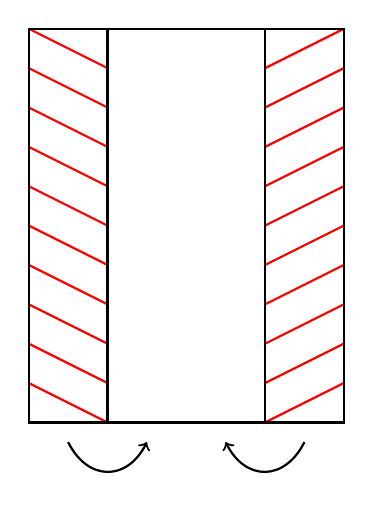
\begin{tikzpicture}[scale=1,
            color=black, fill=black!10, thick,
            cut/.style={color=red}
        ]
            \draw[cut] (0,5.0) -- (1,4.5);
            \draw[cut] (0,4.5) -- (1,4.0);
            \draw[cut] (0,4.0) -- (1,3.5);
            \draw[cut] (0,3.5) -- (1,3.0);
            \draw[cut] (0,3.0) -- (1,2.5);
            \draw[cut] (0,2.5) -- (1,2.0);
            \draw[cut] (0,2.0) -- (1,1.5);
            \draw[cut] (0,1.5) -- (1,1.0);
            \draw[cut] (0,1.0) -- (1,0.5);
            \draw[cut] (0,0.5) -- (1,0.0);

            \draw[cut] (3,4.5) -- (4,5.0);
            \draw[cut] (3,4.0) -- (4,4.5);
            \draw[cut] (3,3.5) -- (4,4.0);
            \draw[cut] (3,3.0) -- (4,3.5);
            \draw[cut] (3,2.5) -- (4,3.0);
            \draw[cut] (3,2.0) -- (4,2.5);
            \draw[cut] (3,1.5) -- (4,2.0);
            \draw[cut] (3,1.0) -- (4,1.5);
            \draw[cut] (3,0.5) -- (4,1.0);
            \draw[cut] (3,0.0) -- (4,0.5);

            % box - needs to be drawn on top of red lines
            \draw (0,0) -- (4,0) -- (4,5) -- (0,5) -- cycle;
            \draw (1,0) -- (1,5);
            \draw (3,0) -- (3,5);

            \draw[->] (0.5,-0.25) .. controls (.75, -.75) and (1.25, -.75) .. (1.5, -0.25);
            \draw[->] (3.5,-0.25) .. controls (3.25, -.75) and (2.75, -.75) .. (2.5, -0.25);

            % \filldraw (-.5,0.1) .. controls (-2, 2) and (-2, 3) .. (-.5, 4.9) -- cycle;
            % \filldraw (4.5,0.1) .. controls (6, 2) and (6, 3) .. (4.5, 4.9) -- cycle;
        \end{tikzpicture}
        
        \caption{Tagliare la pasta sfoglia lungo le linee rosse.}
        \label{fig:pollo_jawad:tagli_pasta_sfoglia}
    \end{figure}
\end{recipe}

\begin{recipe}{Focaccia}
    \begin{header}
        \portion{1}[teglia (\textit{500 g)}]
        \source{Daniele Traversaro}
        \recipedate{Giugno 2023}

        \preparationTime    {\timeM{30}}
        \preparationWait    {\timeH{2-4}}
        \bakingTimeFan      {\timeM{15-20}}{180}
    \end{header}
    
    \begin{ingredients}[13]
        \ingredientSection{Impasto}
        \ingredient[400][g]{Farina}
        \ingredient[250][g]{Acqua \textit{(tiepida)}}
        \ingredient[9][g]{Sale}
        \ingredient[25][g]{Olio EVO}
        \ingredient[12][g]{Lievito fresco}
        \ingredient[1][cucchiaino]{Zucchero}

        \ingredientSection{Salamoia}
        \ingredient[150][g]{Acqua}
        \ingredient[25][g]{Olio EVO}
        \ingredient{Sale}
    \end{ingredients}
    
    \begin{preparation}
        \step Prepare impasto.
        \step Lasciarlo riposare per \timeM{15} coperto da un canovaccio umido.
        \step Ripiegare impasto su se stesso un paio di volte.
        \step Ungere la teglia.
        \step Mettere l'impasto sulla teglia, lasciarlo lievitare in forno spento per \timeM{60}.
        \step \textit{Controllare che la teglia sia ancora adeguatamente unta}.
        \step Schiacciare l'impasto per coprire tutta la teglia.
        \step Lasciare lievitare in forno per \timeM{30}.
        \step Fare i buchi con le dita, cospargere con tutta la salamoia.
        \step Lasciare lievitare in forno per \timeM{60}.
        \step Cuocere in forno preriscaldato.
    \end{preparation}
\end{recipe}

\begin{recipe}{Kebab}
    \begin{header}
        \portion{3}
        \source{Jawad Shurrush}
        \recipedate{15 Luglio 2023}

        \preparationTime     {\timeM{30}}
        \bakingTimeTop       {\timeM{40-50}}{200}[Grill]
        \bakingTimeTop       {\timeM{10-15}}{200}[Grill - Se si aggiunge la salsa nel forno]
    \end{header}

    \begin{introduction}
        Quello che noi chiamiamo comunemente Kebab si chiama in realtà Shawarma.
    \end{introduction}

    \begin{ingredients}[15]
        \ingredient[750][g]{Tritato bovino}
        \ingredient[\tilde 75][g]{Prezzemolo}
        \ingredient[1 \sfrac{1}{2}]{Cipolle}
        \ingredient{Sale}
        \ingredient{Pepe}
        \ingredient{Pepe inglese}
        \ingredient{Noce moscata}
        \ingredient{Cannella}
        
        \ingredientSection{Salsa}
        \ingredient[250][g]{Salsa Tahini}
        \ingredient[1][limone]{Succo di limone}
        \ingredient{Sale}
        \ingredient{Acqua}
        \ingredientSection*{Facoltativo}
        \ingredient{Prezzemolo}
        \ingredient{Aglio}
        \ingredient{Pomodorini}
    \end{ingredients}

    \begin{preparation}
        \step Tagliare cipolle a pezzi grossi (circa 1 cm).
        \step Tagliare prezzemolo in modo fine.
        \step Unire prezzemolo, cipolle, spezie e carne. Amalgamarle per bene.
        \step Disporre la carne a forma di `dita' su un testo. Usare carta forno ed un leggero strato di olio.
        \step Cuocere in forno.
        \step (Opzionale) Aggiungere sala Tahini sulla carna quando è pronta. Cuocere per altri \timeM{5}.
        \step*
        \step*
    \end{preparation}

    \begin{preparation}[Salsa Tahini]
        \par \textit{Vedi \linkRecipe{tahini}[Salsa Tahini].}
        
        \step Mettere salsa Tahini, eventuali spezie opzionali, succo di limone ed acqua.
        \step Mescolare e correggere fino a raggiungimento di una consistenza ottimale.
    \end{preparation}

    \begin{suggestion}
        \suggestionMark La salsa Tahini si può sia mettere in forno che mangiare a parte dopo.
        \suggestionMark Se la salsa si mette in forno, deve avere una consistenza abbastanza liquida (tipo Yoghurt). 
    \end{suggestion}
\end{recipe}

\begin{recipe}{Pollo all'aglio}
    \begin{header}
        \portion{2+}
        \source{Jawad Shurrush \& Davide Ponzini}
        \recipedate{Luglio 2023}

        \preparationTime     {\timeM{15}}
        \cookingTime         {\timeM{15}}{Fiamma media}
    \end{header}

    \begin{ingredients}[10]
        \ingredient[400][g]{Petto di pollo a fettine}
        \ingredient[300][g]{Pomodori ciliegini}
        \ingredient[5-6][spicchi]{Aglio[]}
        \ingredient{Sale}
        \ingredient{Pepe}
        \ingredient{Cannella}
        \ingredient{Noce moscata}
        \ingredient{Pepe inglese}
        \ingredient{Paprika}
        \ingredient{Peperoncino}
        \ingredient{Olio}

        \ingredientSection{Opzionale}
        \ingredient{Peperoni}
        
        \ingredientSection{Alla fine}
        \ingredient[15][g]{Burro}
        \ingredient[1][limone]{Succo di limone}
    \end{ingredients}

    \begin{preparation}
        \step Soffriggere pollo nell'olio.
        \step Aggiungere le verdure quando la carne prende colore.
        \step Aggiungere spezie a metà cottura.
        \step Aggiungere aglio ad \sfrac{2}{3} della cottura.
        \step Aggiungere burro, far rosolare un attimo.
        \step Aggiungere limone a fine cottura, far rosolare un attimo.
    \end{preparation}

    \begin{suggestion}[3cm]
        \suggestionMark Si consiglia di unirlo al \linkRecipe{risoJawad}[Riso con pastina allo zafferano].
        
    \end{suggestion}
\end{recipe}

\begin{recipe}{Spiedini di tritato}
    \begin{header}
        \portion{5-6}[spiedini]
        \source{Davide Ponzini}
        \recipedate{18 Luglio 2023}

        \preparationTime     {\timeM{15}}
        \cookingTime         {\timeM{5}}{Fiamma bassa}
    \end{header}

    \begin{ingredients}[5]
        \ingredient[200][g]{Tritato bovino}
        \ingredient[150][g]{Prosciutto crudo \textit{(oppure speck)}}
        \ingredient{Sale}
        \ingredient{Pepe}
        \ingredient{Spezie per carni}
        \ingredient{Formaggio}
        \ingredient*{Spiedini}
    \end{ingredients}

    \begin{preparation}
        \step Mescolare tritato con formaggio e spezie.
        \step Disporre in rotoli, infilare spiedini.
        \step Friggere in 1 cm di olio di semi.
    \end{preparation}

    \begin{hint}
        Ricetta ispirata ad un piatto mangiato da Marco Daga.
    \end{hint}
\end{recipe}

\begin{recipe}[label=uova_sode]{Uova sode}
    \begin{header}
        \source{Jawad Shurrush}
        \recipedate{19 Luglio 2023}

        \cookingTime         {\timeM{8}}{Fiamma alta}
    \end{header}

    \begin{ingredients}
        \ingredient{Uova}
    \end{ingredients}

    \begin{preparation}
        \step Riempire pentolino di acqua e mettere uova.
        \step Far bollire acqua; iniziare a contare il tempo indicato da quando bolle.
        \step A fine cottura rimuoverle e passare subito sotto l'acqua fredda.
        \step Togliere il guscio.
    \end{preparation}
\end{recipe}

\begin{recipe}{Piselli con uova}
    \begin{header}
        \portion{1}
        \source{Abbate Maria Luisa}
        \recipedate{Agosto 2023}

        \preparationTime     {\timeM{5}}
        \cookingTime         {\timeM{15}}{Fiamma media}
    \end{header}

    \begin{ingredients}
        \ingredient[200][g]{Piselli}
        \ingredient[\sfrac{1}{2}]{Cipolla}
        \ingredient[2]{Uova}
        \ingredient{Sale}
        \ingredient{Olio}
        \ingredient{Pepe}
        \ingredient[1]{Dado \textit{(opzionale)}}
    \end{ingredients}

    \begin{preparation}
        \step Soffriggere cipolla tagliata.
        \step Aggiungere piselli e coprirli con acqua. Aggiungere dado. Chiudere padella con coperchio.
         \step Lasciare cuocere fino a che i piselli non sono pronti.
        \step Aggiungere uova e cuocerle fino a quanto desiderato. Opzionalemente, mescolare gli albumi con i piselli, facendo attenzione a non toccare i tuorli.
    \end{preparation}
\end{recipe}

\begin{recipe}[label=omelette]{Omelette}
    \begin{header}
        \portion{1}
        \source{Internet}
        \recipedate{12 Agosto 2023}

        \preparationTime     {\timeM{5}}
        \cookingTime         {\timeM{5?}}{Fiamma media}
    \end{header}

    \begin{ingredients}
        \ingredient[2]{Uova}
        \ingredient[30][g]{Latte}

        \ingredientSection{Ripieno}
        \ingredient[2][fette]{Prosciutto cotto}
        \ingredient{Formaggio}
        
        \ingredientSection{Altro}
        \ingredient{Olio}
        \ingredient*{Padella abbastanza larga}
    \end{ingredients}

    \begin{preparation}
        \step Sbattere le uova e mescolarle col latte.
        \step Ungere la padella e far scaldare l'olio.
        \step Mettere il composto in padella ed allargarlo in modo da coprire l'intera superficie.
        \step Una volta che si è compattato, aggiungere su metà il ripieno e richiudere usando con attenzione la spatola.
        \step Terminare la cottura e servire.
    \end{preparation}
\end{recipe}


\fakesection{Salse}[Ragù]
\begin{recipe}{Ragù}
    \begin{header}
        \portion{\tilde 10}[barattoli da 500 ml]
        \source{Samuele Daga \textit{(modificata)}}
        \recipedate{\tilde 2016}
    
        \preparationTime{\timeM{45}}
        \cookingTime{\timeH{3-4}}{Fiamma bassa}
    \end{header}
    
    \begin{ingredients}[10]
        \ingredient{Olio}
        \ingredient[50][g]{Burro}
        \ingredient[15][g]{Aglio}
        \ingredient[100][g]{Cipolla}
        \ingredient[300][g]{Carote}
        \ingredient[100][g]{Sedano}
        \ingredient[1][kg]{Tritato bovino}
        \ingredient{Pepe}
        \ingredient{Sale}
        \ingredient[4][bottiglie]{Salsa di pomodoro}
        \ingredient[2][bicchieri]{Vino rosso corposo}
    \end{ingredients}
    
    \begin{preparation}
        \step Sciogliere burro ed olio in pentola.
        \step Tritare verdure.
        \step Cuocere verdure fino a che non diventano morbide (\timeM{\tilde{}10}).
        \step Aggiungere tritato e pepe.
        \step Cuocere fino a che carne non cambia bene colore (\timeM{\tilde{}10}).
        \step Aggiungere vino.
        \step Cuocere fino a che non si è un po' asciugato (\timeM{\tilde{}15}).
        \step Aggiungere salsa.
        \step Cuocere per \timeH{3-4}.
    \end{preparation}
    
    \begin{suggestion}
        \suggestionMark Usare pentola con fondo antiaderente per non bruciare il fondo.
        \suggestionMark Non aggiungere olio dopo la carne, brucia il fondo in ogni caso.
    \end{suggestion}
    
    \begin{hint}
        Grazie Sammy per avermi fatto iniziare a cucinare!
    \end{hint}
\end{recipe}

\begin{recipe}[label=ragu]{Ragù 2.0}
    \begin{header}
        \portion{\tilde 12}[barattoli da 500 ml]
        \source{Davide Ponzini}
        \recipedate{\tilde Marzo 2023}
    
        \preparationTime{\timeM{45}}
        \cookingTime{\timeH{3-4}}{Fiamma bassa}
    \end{header}
    
    \begin{ingredients}[10]
        \ingredient{Olio}
        \ingredient[125][g]{Burro}
        \ingredientSection{Verdure}
        \ingredient[40][g]{Aglio}
        \ingredient[250][g]{Cipolla}
        \ingredient[750][g]{Carote}
        \ingredient[250][g]{Sedano}
        \ingredientSection{Carne}
        \ingredient[1000][g]{Tritato bovino}
        \ingredient[1000][g]{Tritato bovino}
        \ingredient[500][g]{Mortadella tritata}
        \ingredient{Sale}
        \ingredientSection{Altro}
        \ingredient[5.5][g]{Pepe nero}
        \ingredient[5][bottiglie]{Salsa di pomodoro}
        \ingredient[1\sfrac{1}{4}][bottiglie]{Vino rosso corposo}
    \end{ingredients}
    
    \begin{preparation}
        \step Sciogliere burro ed olio in pentola.
        \step Tritare verdure.
        \step Cuocere verdure fino a che non diventano morbide (\timeM{\tilde{}10}).
        \step Aggiungere tritato e pepe.
        \step Cuocere fino a che carne non cambia bene colore (\timeM{\tilde{}10}).
        \step Aggiungere vino.
        \step Cuocere fino a che non si è un po' asciugato (\timeM{\tilde{}15}).
        \step Aggiungere salsa.
        \step Cuocere per \timeH{3-4}.
    \end{preparation}
    
    \begin{suggestion}[1cm]
        \suggestionMark Usare pentola con fondo antiaderente per non bruciare il fondo.
        \suggestionMark Non aggiungere olio dopo la carne, brucia il fondo in ogni caso.
    \end{suggestion}
    
    \begin{hint}
        Ricetta migliorata grazie ai proff. del Marco Polo.
    \end{hint}
    
\end{recipe}

\begin{recipe}[label=besciamella]{Besciamella}
    \begin{header}
        \portion{??}
        \source{Abbate Maria Luisa}
    
        \preparationTime{\timeM{??}}
        \cookingTime{\timeM{??}}{Fiamma bassa+}
    \end{header}
    
    
    \begin{ingredients}
        \ingredient[1][l]{Latte}
        \ingredient{Farina}
        \ingredient[60-70][g]{Burro}
        \ingredient[1][manciata]{Sale}
        \ingredient[1][cucchiaio raso]{Noce moscata}
    \end{ingredients}
    
    \begin{preparation}
        \step Bollire latte con burro, sale, noce moscata.
        \step Quando il latte è caldo ed il burro sciolto, mettere farina (setacciandola).
        \step Mescolare man mano con una frusta.
        \step Continuare a miscelare fino a che è tiepida, se no si formano grumi.
    \end{preparation}
    
    \begin{suggestion}
        \suggestionMark Usare una pentola \underline{non} antiaderente.
        \suggestionMark Se sta vendendo troppo densa, aggiungere latte.
    \end{suggestion}
\end{recipe}

\begin{recipe}{Salsa Barbeque}
    \begin{header}
        \portion{500+}[ml]
        \source{Samuele Daga}
        \recipedate{\tilde 2018}
    
        \preparationTime{\timeM{10}}
        \cookingTime{\timeM{20}}{Fiamma bassa}
    \end{header}
    
    \begin{ingredients}[10]
        \ingredient[300/350][g]{Salsa pomodoro}
        \ingredient[10][g]{Concentrato pomodoro}
        \ingredient[60][g]{Aceto bianco}
        \ingredient[40][g]{Burro}
        \ingredient[100][g]{Cipolla}
        \ingredient[10][g]{Senape}
        \ingredient[100][g]{Zucchero di canna}
        \ingredient{Sale}
        \ingredient[Poco]{Pepe}
        \ingredient{Salsa Worchestershire}
        \ingredient[Molto poca]{Salsa Tabasco}
        \ingredient[10][g]{Peperoncino}
        \ingredientSection{Opzionale}
        \ingredient[1][g]{Peperoncino in polvere}
    \end{ingredients}
    
    \begin{preparation}
        \step Tritare cipolla, far soffriggere in burro a fiamma alta.
        \step Aggiungere aceto, sfumare.
        \step Aggiungere salsa e concentrato pomodoro, zucchero senape.
        \step Cuocere a fuoco basso per \timeM{20}.
        \step Setacciare salsa.
        \step Aggiungere Tabasco, Worchestershire, sale, pepe.
        \step Mescolare.
    \end{preparation}
    
    \begin{hint}
        Perfetta per le grigliate. Su gentile concessione di Sam.
    \end{hint}
\end{recipe}

\begin{recipe}{Fonduta di formaggio}
    \begin{header}
        \portion{100 g}[per persona]
        \source{Manuela Del Bianco}
        \recipedate{\tilde 2017}
    
        \preparationTime{\timeM{10}}
        \cookingTime{\timeH{1+}}{Fiamma bassa}
    \end{header}
    
    \begin{introduction}
        Prestare particolare attenzione alla scelta dei formaggi:
        
        \begin{itemize}
            \item Scamorza ok solo senza buccia
            \item Formaggi duri no (non si sciolgono bene)
                \begin{itemize}
                    \item Grana/parmigiano
                    \item Pecorino
                \end{itemize}
        \end{itemize}
    \end{introduction}
    
    \begin{ingredients}
        \ingredient[\sfrac{1}{3}]{Toma piemontese}
        \ingredient[\sfrac{1}{3}]{Raschera}
        \ingredient[\sfrac{1}{3}]{Fontina}
        \ingredient{Latte}
        \ingredient{Noce moscata}
    \end{ingredients}
    
    \begin{preparation}
        \step Tagliare formaggi a cubetti.
        \step Metterli in un pentolino con il latte.
        \step Cuocere a fuoco basso-medio fino a che il latte non bolle.
        \step Aggiungere noce moscata.
        \step Mescolare costantemente per \timeH{1}.
    \end{preparation}
    
    \begin{suggestion}
        \suggestionMark Per far rassodare più velocemente, è possibile aggiungere della farina alla fine.
    \end{suggestion}
\end{recipe}

\begin{recipe}[label=tahini]{Salsa Tahini}
    \begin{header}
        \source{Jawad Shurrush}
        \recipedate{15 Luglio 2023}
    \end{header}
    
    \begin{ingredients}
        \ingredient[250][g]{Salsa Tahini}
        \ingredient[1][limone]{Succo di limone}
        \ingredient{Sale}
        \ingredient{Acqua}
        \ingredientSection*{Facoltativo}
        \ingredient{Prezzemolo}
        \ingredient{Aglio}
        \ingredient{Pomodorini}
    \end{ingredients}

    \begin{preparation}
        \step Mettere salsa Tahini, eventuali spezie opzionali, succo di limone ed acqua.
        \step Mescolare e correggere fino a raggiungimento di una consistenza ottimale.
    \end{preparation}
\end{recipe}


\fakesection{Dolci}[Salame al cioccolato]
\begin{recipe}{Salame al cioccolato}
    \begin{header}[
        \portion{6+}
        \source{Internet}
        \recipedate{\tilde 2019}
    
        \preparationTime{\timeH{1}}
        \preparationWait{\tilde \timeH{8}}[Frigo]
    \end{header}
    
    \begin{ingredients}[5]
        \ingredient[200][g]{Cioccolato fondente}
        \ingredient[200][g]{Biscotti secchi}
        \ingredient[200][g]{Burro}
        \ingredient[200][g]{Zucchero}
        \ingredient[2]{Uova}
        \ingredient[10][g]{Rhum}
        \ingredient{Zucchero a velo}
    \end{ingredients}
    
    \begin{preparation}
        \step Spezzettare biscotti.
        \step Tagliare cioccolato a fette con coltello.
        \step Sciogliere cioccolato a bagnomaria.
        \step Montare burro e zucchero in una ciotola (con un cucchiaio).
        \step Aggiungere rhum. Mescolare.
        \step Aggiungere uova, precedentemente sbattute. Mescolare.
        \step Aggiungere cioccolato fuso. Mescolare.
        \step Aggiungere biscotti. Mescolare.
    \end{preparation}
\end{recipe}

\begin{recipe}{Ginevrini}
    \begin{header}
        \source{Internet}
        \recipedate{\tilde Aprile 2019}
    
        \preparationTime{\timeM{5}}
        \cookingTime{\timeM{5}}{Fiamma bassa}
    \end{header}
    
    \begin{introduction}
        Consigliato:
        
        \begin{itemize}
            \item Spremuta d'arancia + zucchero
            \item Rhum + zucchero
        \end{itemize}
    \end{introduction}
    
    \begin{ingredients}
        \ingredient[4][g]{Zucchero}
        \ingredient[1][g]{Liquido\newline
            (acqua, succo di frutta o liquore)}
    \end{ingredients}
    
    \begin{preparation}
        \step Mettere in un pentolino di acciaio zucchero e liquido.
        \step Far sciogliere a fiamma bassa. \underline{Non far bollire}.
        \step Una volta pronto, usare cucciaino di acciaio per creare gocce su carta forno.
        \step Lasciare prendere aria per \timeD{1-2}.
    \end{preparation}
\end{recipe}

\begin{recipe}{SacherTorte}
    \begin{header}
        \portion{8}
        \source{Internet}
        \recipedate{\tilde 2019}
    
        \preparationTime{\timeH{1}}
        \bakingTimeTopbottom{\timeM{35-40}}{170}
    \end{header}
    
    \begin{ingredients}[15]
        \ingredient[75][g]{Cioccolato fondente}
        \ingredient[3 (90 g)]{Albumi}
        \ingredient[3 (60 g)]{Tuori}
        \ingredient[65][g]{Burro ammorbidito}
        \ingredient[65][g]{Farina 00}
        \ingredient[20][g]{Zucchero a velo}
        \ingredient[90][g]{Zucchero}
        \ingredient[3][g]{Vaniglia}
        \ingredient[1][pizzico]{Sale fino}
        \ingredientSection{Farcitura}
        \ingredient[200][g]{Marmellata albicocche}
        \ingredientSection{Copertura}
        \ingredient[185][g]{Cioccolato fondente}
        \ingredient[125][g]{Panna fresca}
    \end{ingredients}
    
    \begin{preparation}
        \step Fondere cioccolato.
        \step Setacciare farina.
        \step Mescolare burro, zucchero a velo, vaniglia e sale.
        \step Aggiungere tuorli, mescolare fino a che è ben montato (\timeM{8-10}).
        \step Controllare che il cioccolato sia tra \temperature{45} e \temperature{55}.
        \step Aggiungere cioccolato, mescolare.
        \step Montare albumi quasi fino a neve (non deve essere neve ferma).\newline
            Aggiungere lo zucchero piano piano, appena cominciano a montare (non prima o monteranno più a fatica).
        \step Unire albumi al resto, mescolare con spatola.
        \step Aggiungere farina, mescolare.
        \step Imburrare ed infarinare stampo.
        \step Versare composto.
        \step Cuocere in forno a \temperature{170} per \timeM{35-40}.
        \step Controllare con stecchino.
        \step Tagliare torta a metà con coltello a lama seghettata.
        \step Spalmare con spatola marmellata all'interno.
        \step Spalmare con spatola marmellata su superficie (e bordi).
        \step Mettere panna sul fuoco.
        \step Quando bolle aggiungere cioccolato spezzettato.
        \step Girare fino a che è ben amalgamato.
        \step Far raffreddare fino a \temperature{40}.
        \step Ricoprire torta.
        \step Mettere in frigo per almeno \timeM{20}.
    \end{preparation}
    
    \begin{suggestion}
        \suggestionMark Mescolare la ganache con minipimer per eliminare i grumi.
        \suggestionMark Non esagerare con la marmellata.
    \end{suggestion}
    
    \begin{hint}
        CompleManu!
    \end{hint}
\end{recipe}

\begin{recipe}[label=mou]{Caramello Mou}
    \begin{header}
        \portion{100}[g]
        \source{Internet}
        \recipedate{\tilde Aprile 2019}
    
        \preparationTime{\timeM{1}}
        \cookingTime{\timeM{10}}{Fiamma bassa}
    \end{header}
    
    \begin{ingredients}[4]
        \ingredient[200][g]{Zucchero}
        \ingredient[120][g]{Panna fresca}
    \end{ingredients}
    
    \begin{preparation}
        \step Far quasi bollire panna, lasciarla lì.
        \step Mettere in pentolino di acciaio zucchero (e acqua).
        \step Far cuocere a fiamma bassa fino a \temperature{170}.
        \step Unire panna e mescolare con un cucchiaio di acciaio.
    \end{preparation}
    
    \begin{suggestion}
        \suggestionMark Usare pentola molto più grande di quello che sembra.
            Per lavare usare acqua calda.
        
        \suggestionMark Tara confezione: 17g.
    \end{suggestion}
\end{recipe}

\begin{recipe}{Cioccolatini al Mou}
    \begin{header}
        \portion{24}[cioccolatini]
        \source{Internet}
        \recipedate{\tilde Aprile 2019}
    
        \cookingTime{\timeM{5}}{Fiamma bassa}[Cioccolato]
        \preparationTime{\timeM{30}}[Rivestimento esterno]
        \preparationWait{\timeM{20}}
        \preparationTime{\timeM{30}}[Farcitura]
        \preparationWait{\timeH{1}}
        
    \end{header}
    
    \begin{ingredients}
        \ingredient[300][g]{Cioccolato fondente 70\%}
        \ingredient[120][g]{Caramello Mou}
        \ingredient*{Stampini per cioccolatini}
    \end{ingredients}
    
    \begin{preparation}
        \step Preparare \linkRecipe{mou}[Mou].
        \step Far sciogliere cioccolato a bagnomaria.
        \step Mettere negli stampini cioccolato e spennellare i bordi degli stampini per bene.
        \step Mettere stampini in frigo per \timeM{20}.
        \step Aggiungere mou agli stampini, coprire con cioccolato.
        \step Lasciare in frigo per \timeH{1}.
    \end{preparation}
    
    \begin{suggestion}
        \suggestionMark Ricoprire per bene i bordi degli stampini, per evitare si formino buchi.
    \end{suggestion}
    
    \begin{hint}
        Spuntino dei 24 CFU.
    \end{hint}
    
\end{recipe}

\begin{recipe}{Nutellotti}
    \begin{header}
        \portion{25}[biscottini]
        \source{Marta Daga}
        \recipedate{Aprile 2020}
    
        \preparationTime{\timeM{30}}
        \bakingTimeTopbottom{\timeM{10}}{170}
    \end{header}
    
    \begin{ingredients}
        \ingredient[180][g]{Nutella}
        \ingredient[1]{Uova}
        \ingredient[135][g]{Farina 00}
        
        \ingredientSection{Farcitura}
        \ingredient[125][g]{Nutella}
        \ingredient[30][g]{Granella di nocciole}
    \end{ingredients}
    
    \begin{preparation}
        \step Mescolare uovo e Nutella con le fruste per \timeM{2}.
        \step Aggiungere la farina, setacciandola. Mescolare con una spatola.
        \step Creare un panetto, avvolgere nella pellicola, lasciare riposare in frigo per \timeM{15-20}.
        \step Formare tante piccole palline con le mani. Appiattire con le dita il centro di ciascun pezzo.
        \step Mettere la Nutella rimanente in una Sac-a-poche (con bocchetta stellata).
        \step Farcire la cavità creata precedentemente.
        \step Ricoprire con granella di nocciole.
        \step Mettere in forno.
        \step Far raffreddare.
    \end{preparation}
\end{recipe}

\begin{recipe}{Crema di nocciole ``tipo Nutella"}
    \begin{header}
        \portion{1}
        \source{Samuele Data \textit{(rivisitata)}}
        \recipedate{\tilde 2018}
    
        \preparationTime{\timeM{15}}
    \end{header}
    
    \begin{ingredients}
        \ingredient[150][g]{Nocciole tostate}
        \ingredient[$<<$150][g]{Zucchero}
        \ingredient[$>>$75][g]{Miele d'acacia}
        \ingredient[7][g]{Cacao in polvere}
        \ingredient{Zenzero in polvere}
    \end{ingredients}
    
    \begin{preparation}
        \step Tostare le nocciole
        \step Tritare le nocciole fino a che rilasciano l'olio
        \step Aggiungere zucchero, tritare
        \step Aggiungere miele, cacao e zenzero, tritare
    \end{preparation}
\end{recipe}

\begin{recipe}[label=gelato]{Gelato}
    \begin{header}
        \portion{500}[g]
        \source{Abbate Maria Luisa \textit{(modificata}}
        \recipedate{Agosto 2023}

        \preparationWait     {\timeH{12}}   [Congelatore -- vaschette]
        \preparationTime     {\timeM{30}}
    \end{header}

    \begin{ingredients}
        \ingredient[200][ml]{Panna fresca}
        \ingredient[300][ml]{Latte intero fresco}
        \ingredient[100][g]{Zucchero}
        
        \ingredientSection{Gusti vari}
        \ingredient[50][g]{Cocco}
        \ingredient{Cioccolato fondente a scaglie}

        \ingredientSection{Altro}
        \ingredient*{Macchina per i gelati}
        \ingredient*{Planetaria o fruste}
    \end{ingredients}

    \begin{preparation}
        \step Far raffreddare in congelatore le vaschette.
        \step Montare la panna.
        \step Mescolare ad eventuali altri ingredienti.
        \step Azionare la macchina per i gelati e versare il composto.
        \step Aspettare che il gelato abbia raggiunto una consistenza adeguata.
        \step Riporre il preparato nel congelatore.
    \end{preparation}
\end{recipe}


\fakesection{Bevande}[Liquore all'anice]
\begin{recipe}{Liquore all'anice}
    \begin{header}
        \portion{4+}[litri]
        \source{Internet}
        \recipedate{\tilde 2019}
    
        \preparationTime{\timeM{10}}[Ingredienti]
        \preparationWait{\timeD{30}}
        \preparationTime{\timeM{15}}[Sciroppo]
        \preparationWait{\timeH{4}}[Far raffreddare lo sciroppo]
        \preparationWait{\timeD{60}}
    \end{header}

    \begin{ingredients}
        \ingredient[2][L]{Alcohol per liquori}
        \ingredient[2][L]{Acqua}
        \ingredient[1.5][kg]{Zucchero}
        \ingredient[150][g]{Anice stellato}
        \ingredient[15]{Chiodi di garofano}
        \ingredient[5]{Stecche di cannella}
    \end{ingredients}
    
    \begin{preparation}
        \step Mettere in una bottiglia alcohol, anice, chiodi di garofano, cannella.
        \step Lasciare riposare, agitando ogni giorno.
        \step Preparare sciroppo con acqua e zucchero.
        \step Far bollire per \timeM{2}.
        \step Far raffreddare sciroppo.
        \step Unire al liquore.
        \step Lasciare riposare.
    \end{preparation}
    
    \begin{suggestion}
        \suggestionMark Il liquore migliora di sapore dopo un po' di tempo. Si consiglia di farlo riposare ben oltre il tempo indicato.
        
        \suggestionMark Costo stimato di produzione: \tilde 10.37€/litro\footnote{
            Marzo 2023.
            Consultare codice sorgente commentato per informazioni dettagliate.
            % stecche cannella       2.36 €
            % chiodi di garofano     0.14 €
            % anice                ~ 3.00 € (comprato da Jawad, in Italia anche 60€/kg)
            % alcohol               33.80 €
            % zucchero               2.17 €
            % acqua                    -- €
            % _______________________________________
            % totale                41.47 € per 4 lt
            %  
            % escluse dal conteggio:
            %       bottiglie        4.29 € (aranciata Lurisia, 0.275 lt/bottiglia)
        }.
    \end{suggestion}
\end{recipe}


\fakesection{Varie}[Nocciole tostate]
\begin{recipe}{Nocciole tostate}
    \begin{ingredients}
        \ingredient{Nocciole}
    \end{ingredients}
    
    \begin{preparation}
        \step Mettere le nocciole in forno preriscaldato.
        \step Dopo \timeM{5} spegnere e lasciare raffreddare dentro al forno.
    \end{preparation}
\end{recipe}

\begin{recipe*}{Spezie per carni}
    \begin{ingredients*}
        \ingredient{Sale}
        \ingredient{Rosmarino}
        \ingredient{Origano}
        \ingredient{Pepe}
        \ingredient{Salvia}
        \ingredient{Ginepro}
        \ingredient{Prezzemolo}
        \ingredient{Aglio}
    \end{ingredients*}
\end{recipe*}

\begin{recipe}{Spezie per patate}
    \begin{ingredients*}
        \ingredient{Sale}
        \ingredient{Rosmarino}
        \ingredient{Basilico}
        \ingredient{Maggiorana}
        \ingredient{Timo}
        \ingredient{Salvia}
        \ingredient{Ginepro}
        \ingredient{Aglio}
        \ingredient{Alloro}
        \ingredient{Coriandolo}
        \ingredient{Prezzemolo}
        \ingredient{Cipolla}
    \end{ingredients*}
\end{recipe}



% ----------------------------------------------------------------------------------------------------

\end{document}
